\documentclass[tikz, border=5pt]{standalone}
\usepackage{tikz}
\usepackage{pgfplots}
\pgfplotsset{compat=1.18}

% 定义颜色
\definecolor{impcolor}{RGB}{178, 34, 34}
\definecolor{synflowcolor}{RGB}{65, 105, 225}
\definecolor{snipcolor}{RGB}{60, 179, 113}
\definecolor{gridcolor}{RGB}{200, 200, 200}

\begin{document}
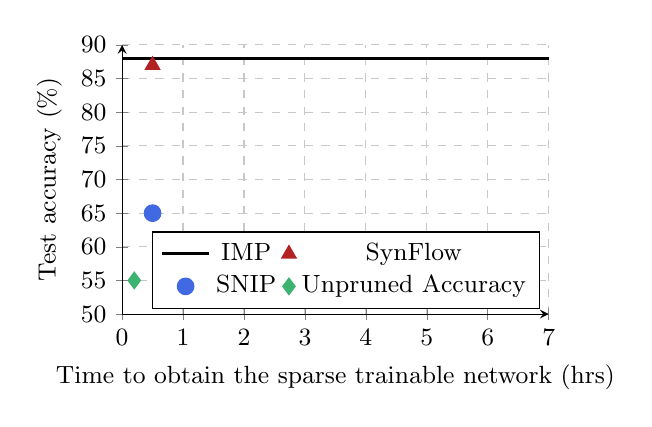
\begin{tikzpicture}
\begin{axis}[
    width=7cm,
    height=5cm,
    xlabel={Time to obtain the sparse trainable network (hrs)},
    ylabel={Test accuracy (\%)},
    xmin=0, xmax=7,
    ymin=50, ymax=90,
    xtick={0,1,2,3,4,5,6,7},
    ytick={50,55,60,65,70,75,80,85,90},
    ymajorgrids=true,
    xmajorgrids=true,
    grid style={dashed, gridcolor},
    legend style={
        at={(0.98,0.02)},
        anchor=south east,
        legend columns=2,
        font=\small
    },
    tick label style={font=\small},
    label style={font=\small},
    axis lines=left,
    clip=false
]

% Unpruned reference line
\addplot[black, line width=1pt] coordinates {(0,88) (7,88)};

% Data points
\addplot[only marks, mark=triangle*, mark size=3pt, impcolor] coordinates {(0.5,87)};
\addplot[only marks, mark=*, mark size=3pt, synflowcolor] coordinates {(0.5,65)};
\addplot[only marks, mark=diamond*, mark size=3pt, snipcolor] coordinates {(0.2,55)};

% Legend entries
\addlegendentry{IMP}
\addlegendentry{SynFlow}
\addlegendentry{SNIP}
\addlegendentry{Unpruned Accuracy}
\end{axis}
\end{tikzpicture}
\end{document}